\section{Auswertung von Haynes \& Shockley}
\subsection{Messung bei Konstanter Abstand}
	Als erstes wurden die einzelnen gemessenen Datenreihen geplottet und mit einer Gaußschen Normalverteilung gefittet. Die verwendete Form ist in Gleichung \ref{Gaus} zu finden.
	\begin{equation}
		f(x) = A \frac{1}{\sqrt{2\pi \sigma^2}} 	\exp\left(-\frac{1}{2}\frac{(x-x_c)^2}{\sigma^2}\right)+h
		\label{Gaus}
	\end{equation}
	Hierfür wurde das Python Paket \verb|scipy.optimize| mit der Funktion \verb|curve_fit| verwendet. Die Bilder der Messungen sind im Anhang.
	Die Erhaltenen Parameter wurden ohne Offset $h$ abgebildet in Abbildung \ref{SpannungGaus} dargestellt.	Wenn man die Gaußkurve mit der Differentialgleichung \ref{DifferentialGL} welche die Bewegung der Elektronenwolken in Halbleiter beschriebt, vergleicht
	\begin{equation}
		c(t,x)=C\exp\left(-\frac{t}{\tau_n}\right)\cdot\exp\left(-\frac{(x-\mu_nEt	)^2}{4D_nt}\right)
		\label{DifferentialGL}
	\end{equation}
	erhält man folgende Gleichungen für die einzelnen Parameter der Gaußkurve \ref{Gaus}:
	\begin{equation}
		x_c(t)=\mu_nEt \qquad A(t)=\exp\left(-\frac{t}{\tau_n}\right) \qquad \sigma(t)^2=2D_nt
	\end{equation}
	Hierbei sind $\mu_n$ die Beweglichkeit der Elektronenwolken, $\tau_n$ ihre Lebenszeit und $D_n$ die Diffusionskonstante.\par
	\FloatBarrier
	\begin{figure}[ht]
		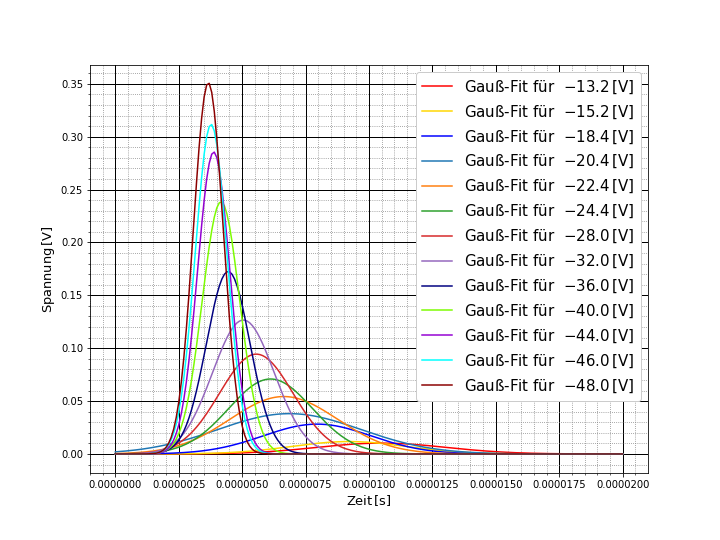
\includegraphics[scale=0.45]{Bild/V2Abstand1}
		\centering
		\caption[Darstellung der Gaußkurven bei konst. Abstand]{Gemeinsame Darstellung der Gaußkurven bei konstanten Abstand ohne Offset nebeneinander.}
		\label{SpannungGaus}
	\end{figure}
	\FloatBarrier
	Als erstes wird versucht die Beweglichkeit $\mu_n$ zu bestimmen. Hierfür wurde die Inverse Spannung $\frac{1}{U(t)}$ gegen die Zeit geplottet und mit einer gewichteten linearen Regression gefittet. Als Fehler wurden die Fehler der Zeit auf der y-Achse verwendet. Siehe Abbildung \ref{SpannungBew}. Das multiplizieren der Steigung $m$ mit der Länge des Halbleiters $l=3$\,cm so wie dem Abstand zwischen Laser und Nadel $d=3.6$\,mm ergibt nun die gesuchte Beweglichkeit.
	\begin{equation}
		\mu_1=ldm
	\end{equation}
	Der Fehler ergibt sich durch Gaußsche Fehlerfortpflanzung mit der Gleichung \ref{FFS1} wo bei die Fehler auf die Abstände beide auf $0.1$\,mm geschätzt wurden.
	\begin{equation}
		\sigma_{\mu_1}=\sqrt{\left(dm\sigma_l\right)^2+\left(lm\sigma_d\right)^2+\left(dl\sigma_m\right)^2}
		\label{FFS1}
	\end{equation}
	Dies ergab einen Wert von $\mu_1=\left(3.90 \pm 0.07\right) \times 10^{3}\,\frac{\text{cm}^2}{\text{Vs}}$
	Nun wurde die Lebenszeit über die Amplitude der Gaußfits bestimmt. Hierfür wurde als Amplitude $A \frac{1}{\sqrt{2\pi \sigma^2}}$ verwendet und dies gegen die Zeit geplottet. Die Datenpunkte wurden dann wie in Abbildung \ref{SpannungTau} zu sehen exponentiell gefittet mit der Form \ref{Expotentialform}.
	\begin{equation}
		f(x)=C\exp\left(-\frac{t}{\tau}\right)+h
		\label{Expotentialform}
	\end{equation}
	Für den Parameter und damit die Lebenszeit ergab sich ein Wert von $\tau_1=\left(1.28 \pm 0.08\right) \times 10^{-6}\,s$
	Nun wird die Diffusionskonstante $D_1$ bestimmt, indem $\sigma^2$ gegen die Zeit dargestellt wird und eine linearer Fit an diese Werte angepasst wird (siehe Abbildung \ref{SpannungD}). Da die Fehler auf das Sigma durch das Quadrieren relativ groß wurden wurde ein gewichteter fit mit Fehlern auf $\sigma^2$ durchgeführt. Das halbieren der Steigung des Fits ergibt für die Diffusionskonstante  $D_1=\left(3.4 \pm 0.5\right) \times 10^{-5}
	\,\frac{\text{cm}^2}{\text{s}}$.
	Die Werte sind noch einmal gemeinsam in Tabelle \ref{MesswerteV2} dargestellt, zusammen mit dem erwarteten Literaturwert.
	\FloatBarrier
	\begin{figure}[ht]
		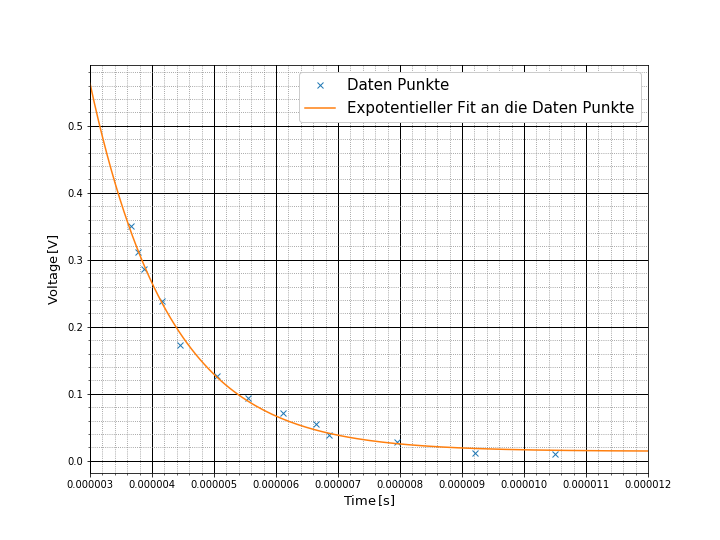
\includegraphics[scale=0.43]{Bild/V2Abstand3}
		\centering
		\caption[Exponentieller Fit der Amplituden bei konstantem Abstand]{\small Exponentieller Fit der Amplituden bei Konstantem Abstand. Fehler wurden nicht eingezeichnet, da sie nicht sinnvoll zu erkennen waren.}
		\label{SpannungTau}
	\end{figure}
	\begin{figure}[ht]
		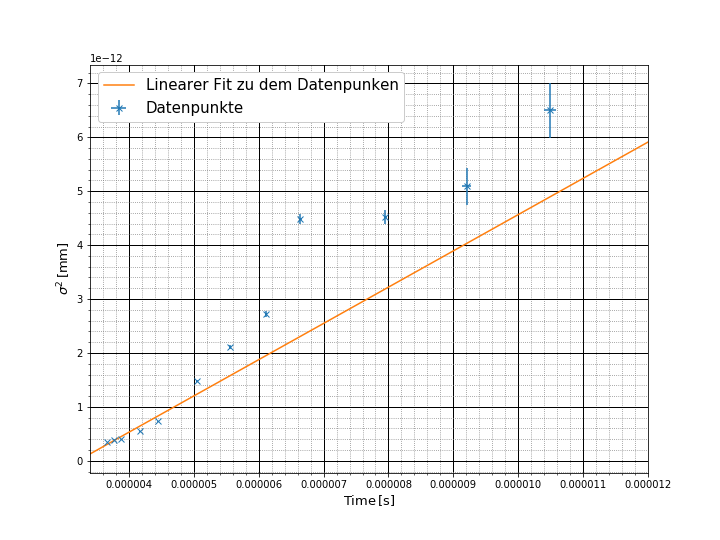
\includegraphics[scale=0.43]{Bild/V2Abstand4}
		\centering
		\caption[Fit zur Bestimmung der Diffusion bei konst. Abstand.]{\small Datenpunkte von $\sigma^2$ gegen die Zeit mit Fehlern. In orange der gerade Fit zur Bestimmung der Diffusionskonstante.}
		\label{SpannungD}
	\end{figure}
	\begin{figure}[ht]
		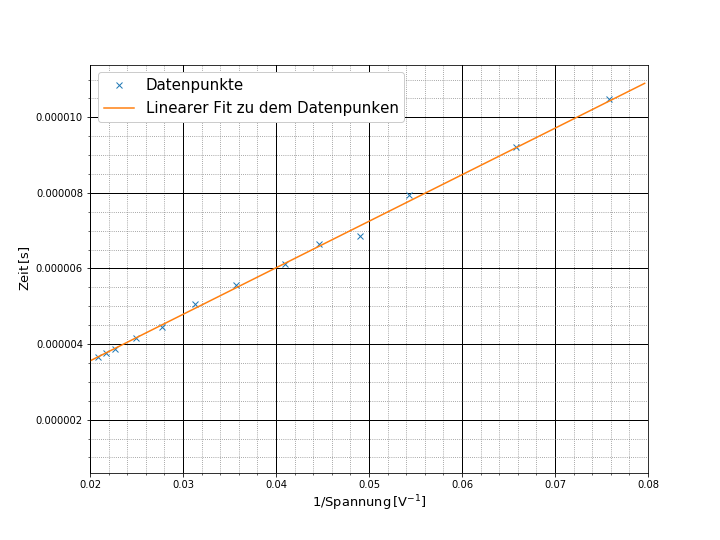
\includegraphics[scale=0.5]{Bild/V2Abstand2}
		\centering
		\caption[Linearer Fit zur Bestimmung der Beweglichkeit bei konst. Abstand]{Linearer Fit zur Bestimmung der Beweglichkeit bei konst. Abstand. Fehler wurden nicht beigefügt, da diese sich nicht sinnvoll darstellen ließen.}
		\label{SpannungBew}
	\end{figure}
	\FloatBarrier
	\newpage
	\subsection{Messung bei Konstante Spannung}
	Für die Messung mit Konstanter Spannung werden wie zuvor die Daten mit der Gleichung \ref{Gaus} gefittet und sind in Abbildung \ref{Abstand1} ohne Offset dargestellt.\par
	\FloatBarrier
	\begin{figure}[ht]
		\includegraphics[scale=0.5]{Bild/V2Spannung1}
		\centering
		\caption[Darstellung der Gaußkurven bei konst. Spannung]{\small Gemeinsame Darstellung der Gaußkurven bei konstanter Spannung ohne Offset nebeneinander.}
		\label{Abstand1}
	\end{figure}
	\FloatBarrier
	Als nächstes wurde die Beweglichkeit $\mu_2$ bestimmt indem der gemessene Abstand zwischen Nadel und Laser gegen die Zeit gefittet, welche die Elektronenwolke benötigte. Hierbei wurden die Fehler auf die Zeit mitberücksichtigt. Die Steigung $m$ erhält man mit Gleichung \ref{AbstandBesch}.
	\begin{equation}
		\mu_2=\frac{1}{mE} \qquad \qquad \sigma_{mu_2}=\sqrt{\left(\frac{\sigma_{m}}{m^2E}\right)^2+\left(\frac{\sigma_{E}}{mE^2}\right)}
		\label{AbstandBesch}
	\end{equation}
	$E$ kann hier über die angelegte Spannung $U=(48\pm0.5)\,$V und die Länge $l=3\pm0.1\,$cm mit Gleichung \ref{E} bestimmt werden.
	\begin{equation}
		E=\frac{U}{l} \qquad \qquad \sigma_E=\sqrt{\left(\frac{\sigma_U}{l}\right)^2+\left(\frac{U\sigma_l}{l^2}\right)^2}
		\label{E}
	\end{equation}
	Damit ergibt sich für $\mu_2=(3136 \pm 32)\,\frac{\text{cm}^2}{Vs}$.\par
	\begin{figure}[ht]
		\includegraphics[scale=0.5]{Bild/V2Spannung2}
		\centering
		\caption[Linearer Fit zur Bestimmung der Beweglichkeit bei konst. Spannung]{\small Linearer Fit zur Bestimmung der Beweglichkeit bei konst. Spannung. Fehler wurden nicht beigefügt, da diese sich nicht sinnvoll darstellen ließen.}
		\label{Abstand}
	\end{figure}
	Danach wird wie bei dem Konstanter Spannung die Lebenszeit wie zuvor über die Amplitude bestimmt. Hierzu wird Gleichung \ref{Expotentialform} benutzt wie in Abbildung \ref{AbstandTau} dargestellt. Für die Lebenszeit ergibt sich dadurch ein Wert von $\tau_2= \left(5.9 \pm 1.0\right) \times 10^{-6}\,s$.\par
	\begin{figure}[ht]
		\includegraphics[scale=0.5]{Bild/V2Spannung3}
		\centering
		\caption[Exponentieller Fit der Amplituden bei konstanter Spannung]{\small Exponentieller Fit der Amplituden bei Konstanter Spannung. Fehler wurden nicht eingezeichnet, da sie nicht sinnvoll zu erkennen waren.}
		\label{AbstandTau}
	\end{figure} 
	Für die Diffusionskonstante wird wieder der Parameter $\sigma^2$ mit Fehlern gegen die Zeit aufgetragen und mit einem gewichteten Fit angepasst. Beide sind in Abbildung \ref{AbstandD}. Es ergibt sich durch halbieren der Steigung ein Wert von $D_2=\left(2.8 \pm 0.7\right) \times 10^{-6}$. Die Werte sind noch einmal gemeinsam in Tabelle \ref{MesswerteV2} dargestellt zusammen mit dem erwarteten Literaturwert.
	\begin{figure}[ht]
		\includegraphics[scale=0.5]{Bild/V2Spannung4}
		\centering
		\caption[Fit zur Bestimmung der Diffusion bei konst. Spannung.]{\small Datenpunkte von $\sigma^2$ gegen die Zeit mit Fehlern. In orange der gerade Fit zur Bestimmung der Diffusionskonstante.}
		\label{AbstandD}
	\end{figure}
	\begin{table}[ht]
		\begin{Dtabular}[1.1]{|c|c|c|c|}
			\hline
			&Beweglichkeit $\mu$ [$\frac{\text{cm}^2}{\text{Vs}}$]&Lebenszeit $\tau$ [$\mu$s]& Diffusion $D$ [$\frac{\text{cm}^2}{\text{s}}$]\\
			\hline
			Messung bei konst. Abstand&$\left(3900 \pm 70\right)$&$\left(1.28 \pm 0.08\right)$&$\left(3.4 \pm 0.5\right) \times 10^{-5}$\\
			\hline
			Messung bei konst. Spannung&$(3136 \pm 32)$&$\left(5.9 \pm 1.0\right)$&$\left(2.8 \pm 0.7\right) \times 10^{-6}$\\
			\hline
			Literaturwert&$3900$&$(45\pm2)$&$101$\\
			\hline
		\end{Dtabular}
		\centering
		\caption{Messwerte von Versuchsteil 2 mit Literaturwerten\cite{anleitung}}
		\label{MesswerteV2}
	\end{table}